\chapter{\leavevmode Introduction}
\label{chap:introduction}

% \section*{Overview}
% \addcontentsline{toc}{section}{Overview}
\section{Overview}  \label{overview}

According to the Federal Trade Commission (FTC), there were 37,932 reports of credit card fraud in 2012 and 87,451 reports in 2022. This marks an increase of credit card payment fraud by an estimated, 30.5\%. By comparison, since 2020, there has been a 14.6\% increase in credit card related fraud. Which does not include the millions of other fraud reports the FTC receives every year. In 2022 alone, there were around 5.1 million fraud, identity theft, and miscellaneous reports in total \autocite{ConsumerSentinelNetwork2023,forthesentinelConsumerSentinelNetwork2022}. The statistics for these reports stresses how crucial the security of payment systems are, both physical and online. And, the need to secure them grows every year.

This research primarily focuses on physical point-of-sale (PoS) systems or terminals and their hardware (serial accessories), rather than online solutions. For instance, not mobile payment apps like Venmo, CashApp, Zelle, or Paypal \autocite{wangMobilePaymentSecurity2016}. There are many reasons, but the types of systems being targeted varies greatly in terms of the hardware and software supported, as well as, how the transactions are handled with the payment processor.

\begin{figure}[ht]%
  \centering
  \subfloat[\centering Square PoS]{{ 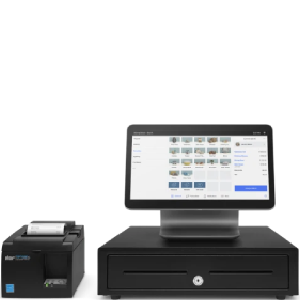
\includegraphics[width=0.50\textwidth,keepaspectratio]{Figures/MidSquare.png} }}%
  \qquad
  \subfloat[\centering SurePoS]{{ 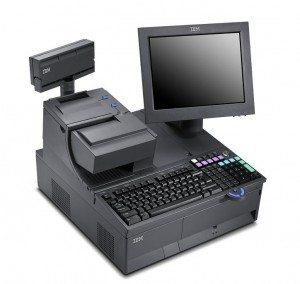
\includegraphics[width=0.40\textwidth,keepaspectratio]{Figures/SurePOS.jpg} }}%
  \caption{Comparison of common PoS systems}%
  \label{fig:comparison_pos}%
\end{figure}

Figure \ref{fig:comparison_pos} shows us two similar looking point-of-sale systems, albeit one is much older looking. However, the operating system and required hardware is very different. Typically, unless you have the Square provided terminal, their software/client is installed onto an Android or iOS device and connected to a Square compatible card reader \autocite{ondrusMobilePaymentsMarket2011}. Whereas, the SurePoS, NCR, or other common EFTPoS system will run a proprietary OS derived from Windows or Linux \autocite{ebimoboweiROLESOFTWARECASHLESS2018}. Furthermore, these PoS tend to require some form of printing receipts as record keeping for the business owner and customer. And these devices also vary in terms of processing capabilities and operating system.

For instance, a common thermal printer seen with PoS systems, integrated with fuel pumps, or other industrial control equipment, is the SNBC BTP-S80 thermal printer \autocite{SNBCBTPS80Thermala,SNBCNewBeiyangIntelligent}. There are multiple versions of the device with support for Bluetooth, USB only, or combination of USB/Serial/Ethernet. The bluetooth hardware is provided over an accessory 25-pin serial connection, with more I/O as a serial connection via RS232C connector and USB Type-B. It has driver support for various platforms: Android, iOS, Windows, Linux, and MacOS. The most interesting aspects are the processor, an Arm Cortex M4 clocked at 3.54MHz, and the operating system, a proprietary version of FreeRTOS. The system architecture is Armv7E-M with JTAG/SWD hardware debugging support \autocite{CortexM4,FreeRTOSMarketLeading}.

By default, the printer has enough headroom to process ESC/POS commands for printing paper and a webserver for debugging or general diagnostics. In theory, the uncompromised device could be flashed with modified firmware to act as a decoy and human-input-device (HID) against the host PoS. In this paper, we propose exploring the processing capabilities and extensibility of FreeRTOS to act as a dual HID clone and printer for continued research. 

\begin{figure}[ht]%
  \centering
  \subfloat[\centering BTP-S80]{{ 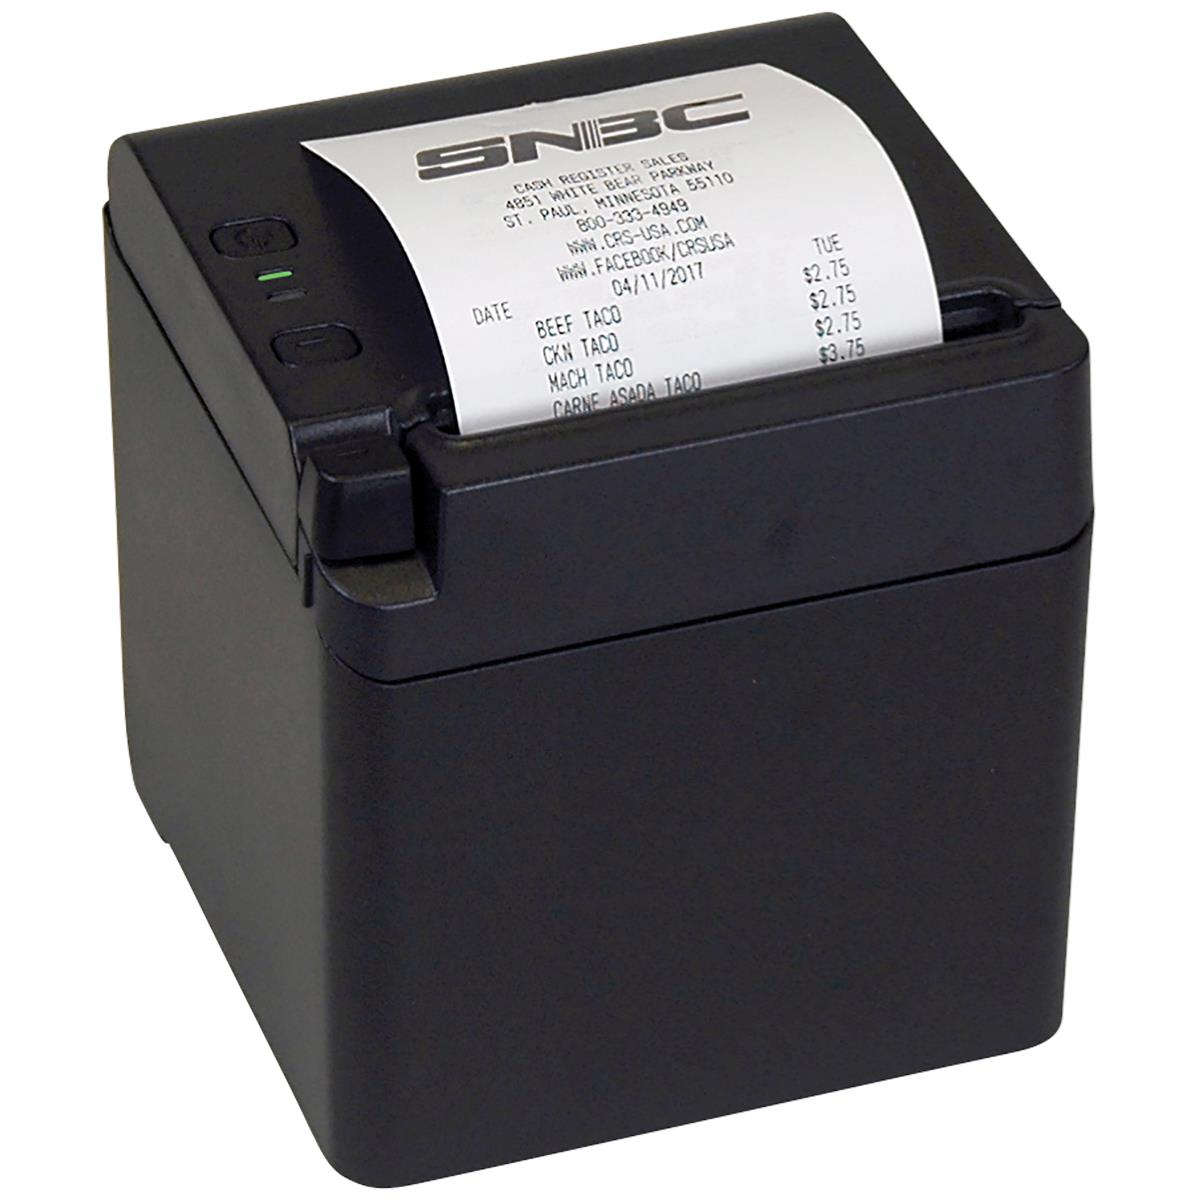
\includegraphics[width=0.40\textwidth,keepaspectratio]{Figures/SNBC_S80.jpeg} }}%
  \qquad
  \subfloat[\centering Printer I/O]{{ 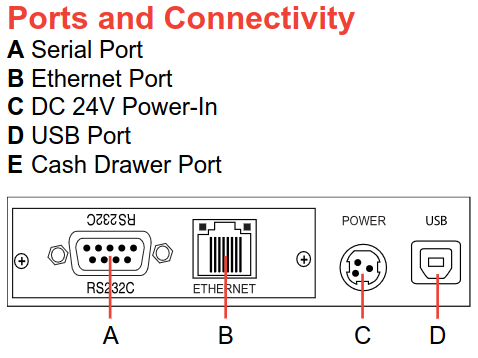
\includegraphics[width=0.40\textwidth,keepaspectratio]{Figures/SNBC_S80_IO.png} }}%
  \caption{SNBC BTP-S80}%
  \label{fig:btp_s80}%
\end{figure}

The goal of this research is to further establish academic works in regards to embedded printer devices testing and security. This area is loosely documented within academia and only mentioned vaguely in relation to statistical reports or applied research using entirely different environments. Through this research we hope to apply gainful conclusions towards the development of an embedded environment for vulnerability assessment, penetration testing, and hardware-to-software interoperability against device hosts. Some examples of how the research could be applied in the future vary: BadUSB/BashBunny \autocite{hak5BashBunny}, JuiceShop \autocite{OWASPJuiceShop}, DVWA \autocite{woodDAMNVULNERABLEWEB2023}, or Webgoat \autocite{OWASPWebGoatOWASP}; no such work exists for embedded systems within the point-of-sale or serial printer context.

% reword this closing paragraph ^ it sucks